\documentclass[10pt]{oblivoir}

% ---------------------------------------------- PACKAGE IMPORTS
\usepackage{kotex}
\usepackage{amsmath}
\usepackage{multicol}
\usepackage{fixltx2e}
\usepackage{float}
\usepackage{graphicx}
\usepackage{fullpage}
\usepackage{siunitx}
\usepackage[ruled,vlined]{algorithm2e}
\usepackage{hyperref}
\usepackage{listings}
\usepackage{color}
\usepackage{caption}
\usepackage{indentfirst}
\usepackage{subcaption}
\usepackage{tikz-cd}
\usepackage{chngcntr}
\usepackage{comment}
\usepackage[nameinlink]{cleveref}

% ---------------------------------------------- FIGURE COUNTER SETTINGS
% \counterwithin{figure}{section}

% ---------------------------------------------- CODE AREA SETTINGS
\definecolor{dkgreen}{rgb}{0,0.6,0}
\definecolor{gray}{rgb}{0.5,0.5,0.5}
\definecolor{mauve}{rgb}{0.58,0,0.82}

\lstset{frame=tb,
  language=C++,
  aboveskip=3mm,
  belowskip=3mm,
  showstringspaces=false,
  columns=flexible,
  basicstyle={\small\ttfamily},
  numbers=none,
  numberstyle=\tiny\color{gray},
  keywordstyle=\color{blue},
  commentstyle=\color{dkgreen},
  stringstyle=\color{mauve},
  breaklines=true,
  breakatwhitespace=true,
  tabsize=3
}

% ---------------------------------------------- CLEVERREF SETTINGS
\crefname{figure}{그림}{그림}
\crefname{equation}{식}{식}
\crefname{table}{표}{표}
\crefname{listing}{목록}{목록}
\crefname{section}{절}{절}
\crefname{algorithm}{알고리즘}{알고리즘}

\captionsetup[subfigure]{subrefformat=simple,labelformat=simple}
    \renewcommand\thesubfigure{ (\alph{subfigure})}

% ---------------------------------------------- GENERAL SETTINGS
\setlength{\parindent}{0.3cm} % The first indent width setup

% ---------------------------------------------- CUSTOM COMMANDS
%       GENERAL
\newcommand{\textss}[1]{\scriptsize#1\normalsize}
%       MATHEMATICAL
\newcommand{\abs}[1]{\left|\,#1\,\right|}

% ---------------------------------------------- HEADER
\title{AR 당구}
\author{강승우 \\ 한국기술교육대학교 전자공학과}
\date{2020.10}

% ---------------------------------------------- CONTENT
\begin{document}
\maketitle

\begin{figure}[ht]
    \centering
    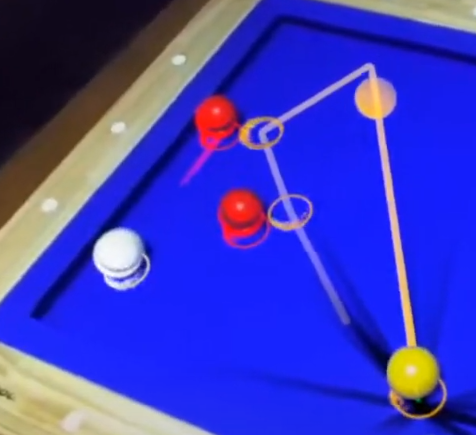
\includegraphics[width=5cm]{img/abstract-final.png}
\end{figure}

\begin{abstract}
    당구는 재미있는 스포츠이지만, 처음 입문한 초심자가 득점 가능한 경로를 계산하고 올바르게 공을 쳐서 보낼 정도로 숙련되기까지의 진입 장벽이 높은 편이다. 당구 초심자가 어느 정도 수준에 도달하기 위해선 지속적인 집중과 훈련을 필요로 하는데, 적절한 동기 부여 요소가 없다면 흥미를 잃어버리기 쉽다. 본 연구는 스테레오 카메라와 VR 카메라를 결합한 몰입도 높은 증강 현실 플랫폼 상에서 당구 경로 안내 및 시각 효과를 통해 초심자의 흥미를 유도하고 당구 학습을 가속하는 것을 목표로 두었다. 이를 위해 OpenCV를 활용하여 당구공 배치를 인식하고 Unity Engine 상에서 물리 시뮬레이션을 통해 경로 탐색과 시각화를 수행하였고, 그 결과 프로그램이 제안한 속도와 방향을 정확히 맞췄을 때 높은 정확도를 보였다. 이는 당구에 처음 입문하는 초심자가 경로 설계에 대한 부담 없이 공을 올바르게 보내는 훈련에만 집중할 수 있게 만들며, 나아가 오랜 시간 알고리즘이 제안하는 경로를 익힘으로써 점진적으로 당구 숙련도를 높일 수 있다는 점에서 AR 당구의 학습 보조 도구로서의 가능성을 확인할 수 있었다.
\end{abstract}

\newpage
\twocolumn[]

\section{서론}
당구는 익숙해지기까지 많은 시간의 훈련과 적응을 필요로 하는 스포츠이다. 정보 매체의 발달로 학습을 필요로 하지 않는 직관적인 오락 컨텐츠가 폭발적으로 양산되는 시대에 이러한 진입 장벽은 초보자들이 발을 들이는 데 어려움으로 작용한다.

당구는 경로 설계와 큐잉(당구공을 큐로 치는 것) 두 가지가 모두 성공적으로 수행되었을 때 득점을 할 수 있다. 그러나 초보자가 나름대로 경로를 설계해 큐잉을 해도, 경로대로 공을 보내는 것 자체가 어려운 만큼 운이 아닌 실력만으로 득점을 내기는 쉽지 않다.

보통 당구는 체계적인 훈련이 아닌 놀이로서 시작하는 경우가 많으며, 놀이로서 학습을 지속하기 위해선 심리적인 보상이 필요하다. 당구에서는 득점이 이에 해당하는데, 상술한 진입 장벽에 빗대어 보면 당구 입문자는 실력이 갖춰질 때까지의 오랜 기간을 확실한 심리적인 보상 없이 훈련을 견뎌야 한다는 이야기가 된다.

% 무득점 = 동기 부여가 어려움
% 학습을 하다 지침

당구공의 경로 안내에 대한 아이디어는 바로 이러한 심리적인 보상 측면에서 출발한다. 아무런 보조 없이 당구를 연습하는 경우 초심자는 경로 설계와 큐잉 양단 모두를 병렬적으로 훈련해 나가야 하는데다 적절한 피드백을 받기도 어려우므로 학습을 지속하기가 어려웠다. 

그러나 득점할 수 있는 경로를 알 수 있다면 초심자는 큐잉에만 온전하게 집중할 수 있으며, 어느 정도 큐잉에 익숙해진 후에는 시스템이 제공하는 경로 정보를 바탕으로 경로 설계에 대한 암시적인 경험을 쌓을 수 있다.

위의 아이디어를 바탕으로 이미 시중에는 당구대 상단에 카메라와 프로젝터를 설치하여 당구공의 배치를 분석해 경로를 안내하거나, 혹은 큐의 방향을 분석해 공의 진행 경로를 예측하는 프로젝트가 소개되었다.
\cite{AR-Pool-Projector} \cite{AR-Pool-Projector-2}

본 연구는 위 프로젝트와 맥락을 같이 하되, 주제의 구현에 점차 보편화되어가고 있는 증강 현실 장비를 활용한다. 이는 기존의 시스템에 비해 장소의 제약이 없는데다, 적은 비용과 높은 범용성을 갖는다. 또한 당구대 평면상에 화면을 투사하는 것이 전부인 기존의 시스템과 달리, 증강 현실 장비는 얼마든지 입체를 표현할 수 있으므로 몰입도 측면에서도 더 뛰어난 경험을 선사할 수 있을 것으로 보인다.

\section{제안 방식}
AR 당구는 다음의 과정으로 동작한다.
\begin{enumerate}
    \item 영상 처리를 통한 당구대, 당구공 포즈 인식
    \item 타격 각도 및 속도 샘플 시뮬레이션으로 득점 경로 계산
    \item AR 카메라의 위치에 따라 선택된 경로 시각화
\end{enumerate}

이 때 영상 처리 프로그램과 물리 연산 및 시각화 프로그램은 각각 OpenCV와 Unity Engine을 활용하기 위해 스트림 소켓으로 데이터를 주고받는 별개의 프로그램으로 작성된다(\cref{fig;overall-proc}). 

하드웨어 플랫폼으로는 Oculus Rift에 Stereolabs의 스테레오 카메라인 ZED Mini를 결합한 AR 장비를 사용하고, 양안 각각 HD(1280$\times$720 해상도) 60FPS로 렌더링을 수행한다.

\begin{figure*}
    \centering
    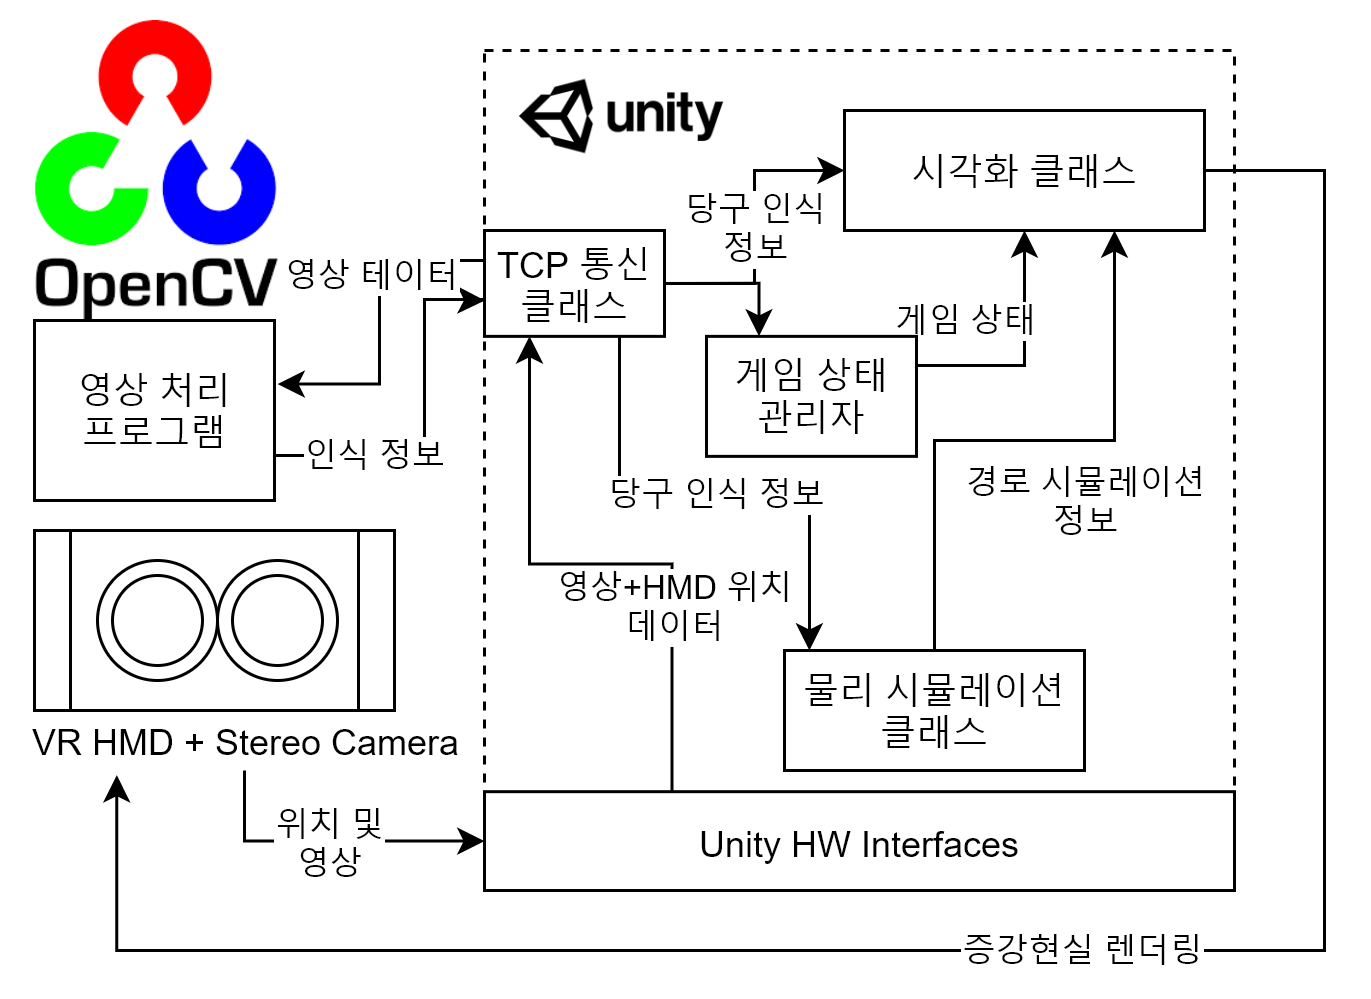
\includegraphics[width=16cm]{img/overall-process.png}
    \caption{전체 과정도}
    \label{fig;overall-proc}
\end{figure*}

\subsection{영상 처리}
% 영상 인식 블록도



% 물리 시뮬레이션 설계 방식

% 시각화 방식

\section{실험 결과}
% 테이블 필터링 과정

% 공 인식 과정

% 물리 시뮬레이션 설계 영상

\section{결론}

\bibliographystyle{ieeetr}
\bibliography{content.bib}

\end{document}
